\documentclass[11pt, oneside]{article}   	% use "amsart" instead of "article" for AMSLaTeX format
\usepackage{geometry}                		% See geometry.pdf to learn the layout options. There are lots.
\geometry{letterpaper}                   		% ... or a4paper or a5paper or ... 
%\geometry{landscape}                		% Activate for for rotated page geometry
%\usepackage[parfill]{parskip}    		% Activate to begin paragraphs with an empty line rather than an indent
\usepackage{graphicx}				% Use pdf, png, jpg, or eps§ with pdflatex; use eps in DVI mode
								% TeX will automatically convert eps --> pdf in pdflatex		
\usepackage{listings}
\usepackage{amssymb}
\usepackage{amsmath}
\usepackage{subfigure}

\lstset{language=Java, basicstyle=\scriptsize}


\title{CS675 Project 2: Get Started with RPC/RMI \\
Performance Evaluation of Game Server Protocols}
\author{Zhonghua Xi}
%\date{}							% Activate to display a given date or no date

\begin{document}
\maketitle

\section{Design}
\subsection{MMORPG}
The game is designed as a MMORPG (Massively multiplayer online role-playing game). Every user will control a role walking on a 2D tiled environment. Each tile can contain a treasure chest (with a random value associated with it) and multiple players. The first player on that tile who opens the chest will be awarded the treasure. After that the treasure will disappear. After all the chest were opened, the game is over, who gets the most score will win the game.

\subsubsection{Control}
Players use keyboard to control the movement of their roles in the virtual space and use space key to open a chest. They will be able to see where treasure boxes and other players are. Users will be notified other players' operations (movement, treasure boxes opened).

\section{Implementation}
\subsection{Server}
Once the server is started, it will generate a new map with treasure chests on the map with random locations and values.

\subsubsection{Socket Based Game Server}
One significant advantage of socket-based game server over RPC/RMI based server is that it can not only push update to each client, it can also broadcast the updates to all clients for certain events. (e.g., a new user entered the world, an existing user left the game)
While the later one can only pull information from server. Thus, besides the required two services (which is not used in socket-based server in practice), I also implemented the push version of the game server. Only changes (any player's location changed, chest opened, etc.) will be pushed to client, client will never call server to get the entire information of the world. This can significantly reduce network overhead (delay) thus improve user's experience.


\subsection{Client}
Once client is started, and connected to server. Then all the information of the world will be either pulled from client or pushed to client. These information will be used to render the world.
Fig.~\ref{fig:world} shows the world map from three different players' viewpoint.
The window title bar shows the current role's location, name and total score awarded.
Each green box in the world represents a treasure chest, each blue dot represents a player and the red dot represents the current player.
From Fig.~\ref{fig:world} we can see all the players were synced with the server.
\begin{figure*}[htbp] %  figure placement: here, top, bottom, or page
   \centering
   \subfigure[Player1]{\fbox{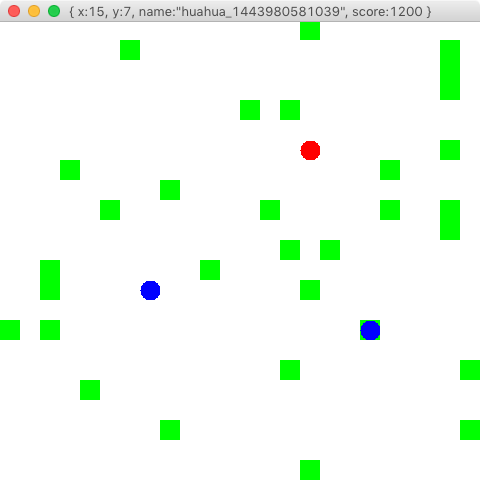
\includegraphics[width=2.8in]{figs/player1.png}}}
   \subfigure[Player2]{\fbox{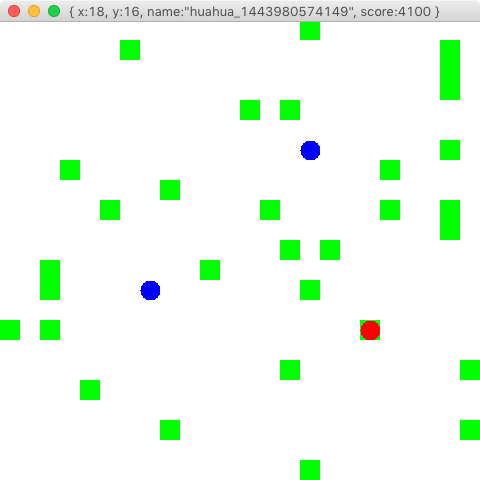
\includegraphics[width=2.8in]{figs/player2.png}}}
   \subfigure[Player3]{\fbox{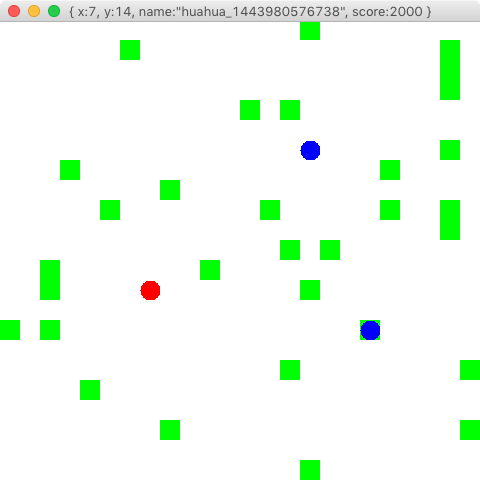
\includegraphics[width=2.8in]{figs/player3.png}}}
   \caption{World from different players' view.}
   \label{fig:world}
\end{figure*} 
%
%\begin{figure}[htbp] %  figure placement: here, top, bottom, or page
%   \centering
%   \subfigure[before peer3 left]{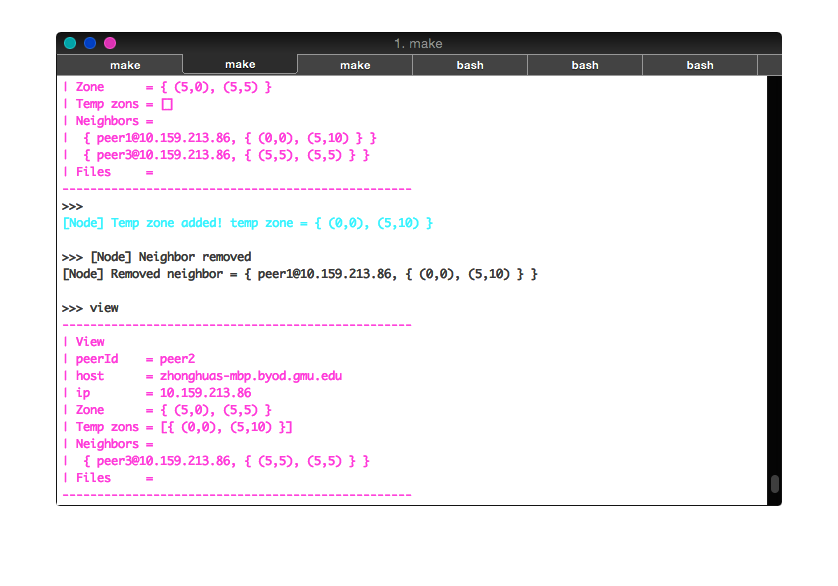
\includegraphics[width=5in, clip=true, trim=22mm 30mm 30mm 28mm]{figures/before.png}}
%   \subfigure[after peer3 left]{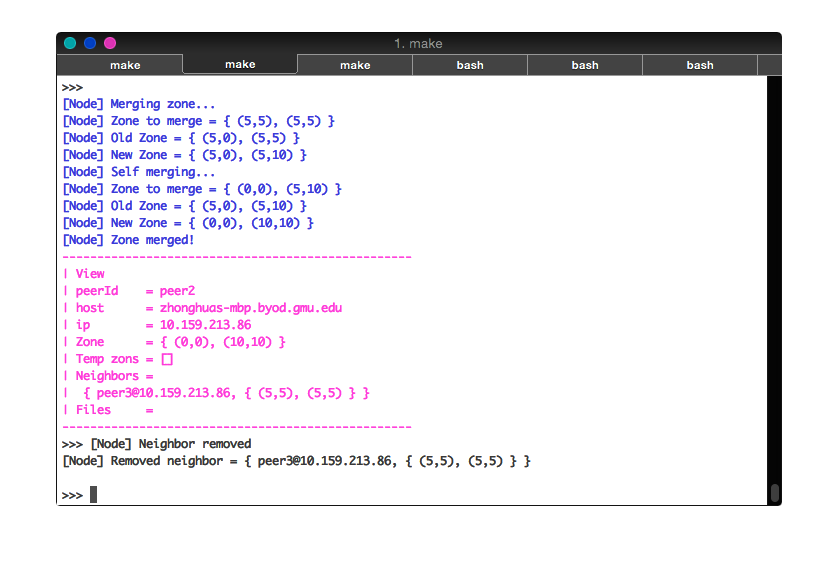
\includegraphics[width=5in, clip=true, trim=22mm 30mm 30mm 28mm]{figures/after.png}}
%   \caption{Screenshots of self-merging process.}
%   \label{fig:screenshot}
%\end{figure} 
%
%\subsection{File Insertion/Retrieval}
%A file is inserted into CAN as a key value pair. Key is the keyword of the file, while the value is the content of the file. The following screenshots show the process of file insertion and retrieval on two nodes.
%
%\begin{figure}[htbp] %  figure placement: here, top, bottom, or page
%   \centering
%      \subfigure[peer1]{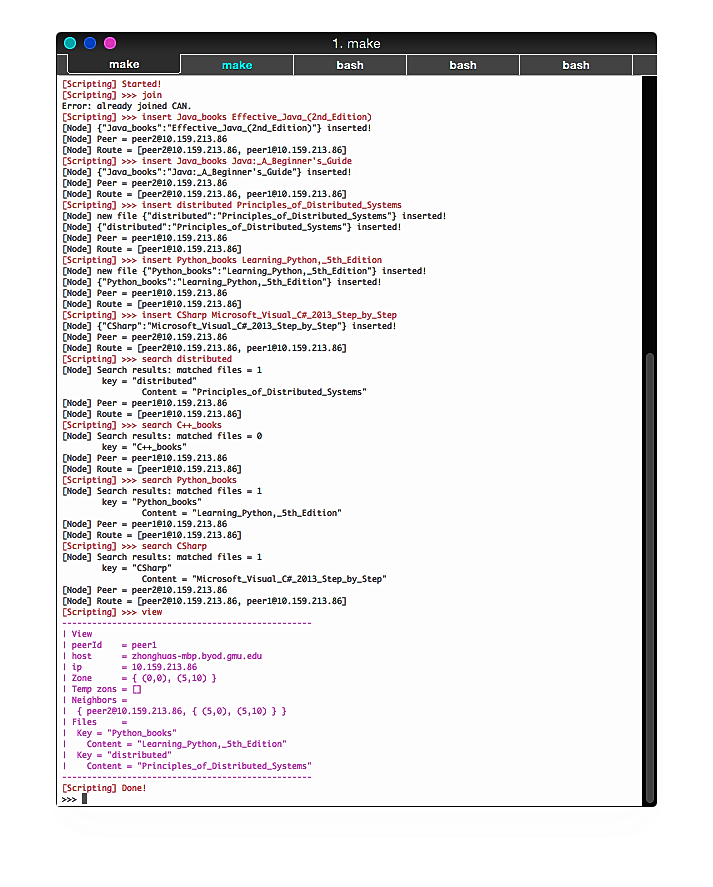
\includegraphics[width=2.9in, clip=true, trim=22mm 29mm 100mm 28mm]{figures/insertion2.png}}
%   \subfigure[peer2]{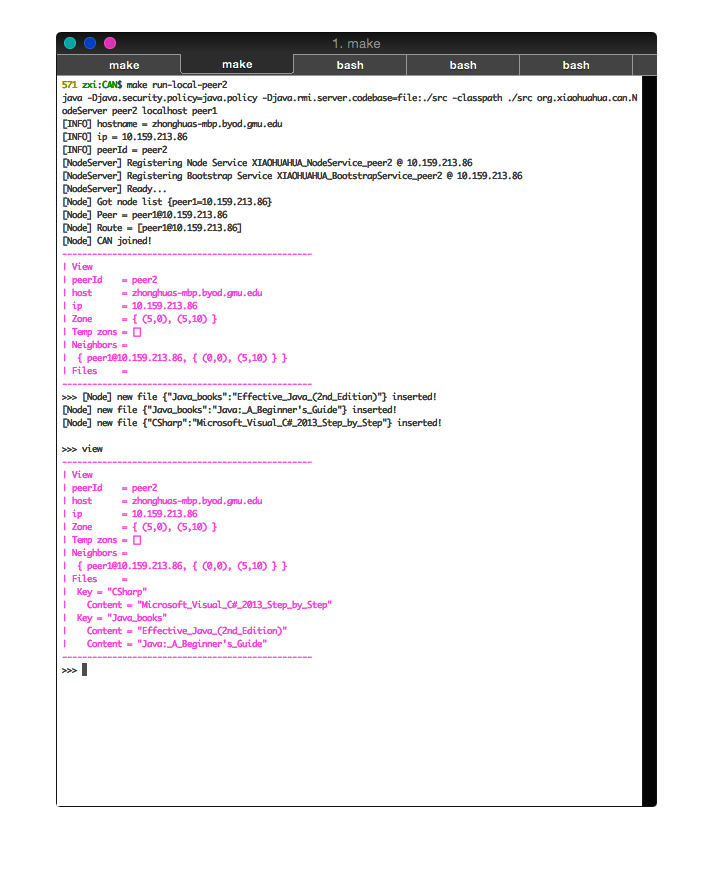
\includegraphics[width=2.9in, clip=true, trim=22mm 29mm 100mm 28mm]{figures/insertion1.png}}
%   \caption{Screenshots of file insertion and retrivel.}
%   \label{fig:insertion}
%\end{figure} 

\end{document}  